\documentclass{article}
\usepackage[spanish]{babel}
\usepackage[utf8]{inputenc}	
\usepackage{graphicx}
\usepackage{mathtools}
\usepackage{vmargin}
\usepackage{pgfplots}
\usepackage{fancyhdr}

\pgfplotsset{compat=newest}
\setpapersize{A4}
\newcommand*\rfrac[2]{{}^{#1}\!/_{#2}}		

\title{Matemática Superior\\Trabajo Práctico 1}

\author{ Busso, Francisco\\francisco.busso@outlook.com 
    \and Ferraro Trivelli, Giovani\\gftrivelli@frsf.utn.edu.ar
    \and Storani, Miguel\\ miguelignaciostorani@gmail.com
}

\pagestyle{fancy}

\renewcommand{\maketitle}{
    \begin{center}
        
        {\scshape{Universidad Tecnológica Nacional\\Facultad Regional Santa Fe}}
        \vspace{10pt}
        \hrule
        \vspace{10pt}
       

        {\LARGE\bfseries{Matemática Superior\\}}
        \vspace{5pt}
        {\Huge\bfseries{Trabajo Práctico 1B}}

        \vspace{8pt}
        \hrule
        \vspace{8pt}

        Busso, Francisco\\
        \textit{francisco.busso@outlook.com}\\
        \vspace{7pt}
        Ferraro Trivelli, Giovani\\
        \textit{gftrivelli@frsf.utn.edu.ar}\\
        \vspace{7pt}
        Storani, Miguel\\
        \textit{miguelignaciostorani@gmail.com}\\

        % Setea el estilo de la pagina a vacío
        \thispagestyle{empty}
        
        % Terimna la pagina actual
        \newpage
    \end{center}
}

\rhead{Matemática Superior}
\lhead{
\includegraphics[width=3.2cm]{logo.png}}

\begin{document}
\maketitle
\newpage

\renewcommand{\contentsname}{Índice}
\tableofcontents
\newpage

    \section{Transformada Discreta}
	\subsection{Visualización de la matriz}

	        \paragraph{}
	        Una vez separada la función en segmentos y calculadas las Transformadas de Fourier en Tiempo Discreto de cada uno, 
	        se construyó la Matriz de Espectro E utilizando la formula propuesta. Posteriormente se determinaron los valores máximo y mínimo de dicha matriz 
	        y se construyó una nueva matriz de igual dimensión a la matriz de espectro, en la cuál se le asignó a cada posición de la misma un valor entre 0 y 255, 
	        mediante la siguiente fórmula:
	
	        \begin{equation}
	            V_{(i, j)}=\frac{E_{(i, j)}-m}{M-m}*255
	        \end{equation}
	
	        Donde \textit{M} representa al valor máximo de la Matriz de Espectro y \textit{m} al valor mínimo de la misma.
	        Esto se realizó para diferenciar gráficamente las frecuencias predominantes (zonas  blancas) 
	        de las frecuencias que aportan menos energía (zonas negras) a la señal final.
	
	        \begin{figure}[h!]
	            \centering
	            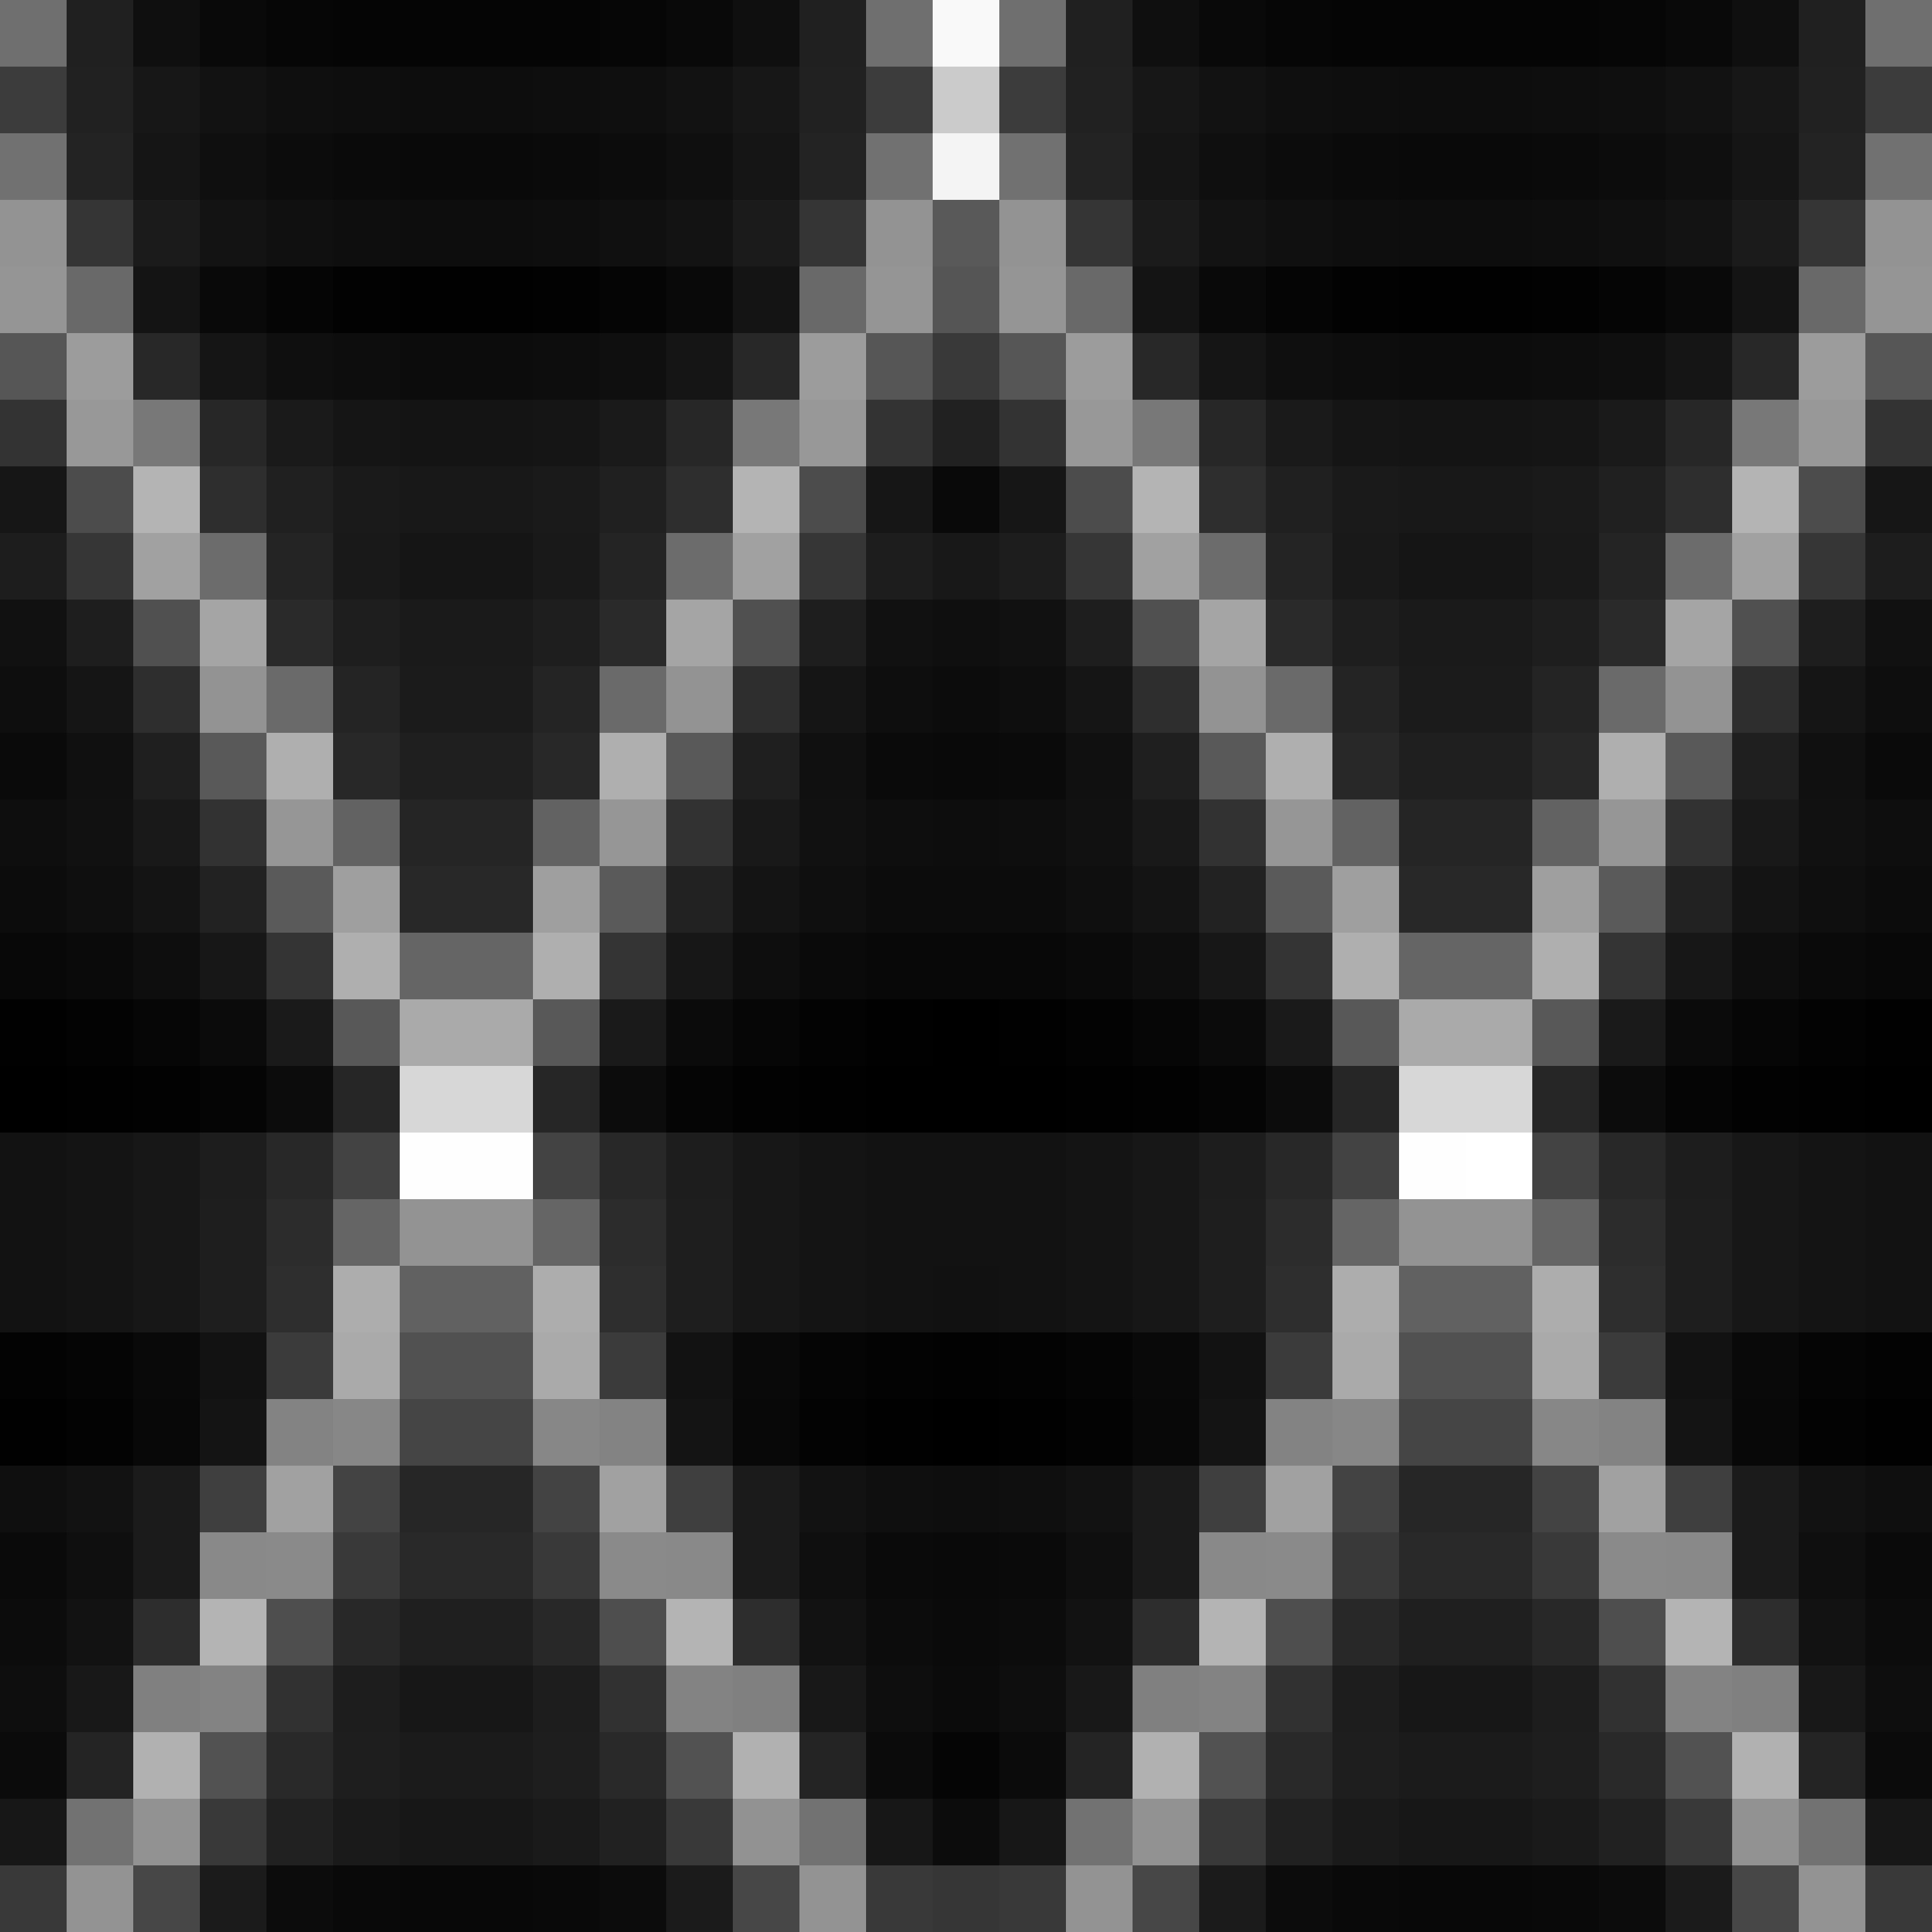
\includegraphics[width=40mm]{color_img}
	            \caption{Representación gráfica de la Matriz de Espectro}
	            \label{imagen1}
	        \end{figure}
	
	        \paragraph{}
	        Lo mismo se realizó para una señal simple de frecuencia constante y para una señal con variación de frecuencia lineal.
	
	        \begin{figure}[h!]
	            \centering
	            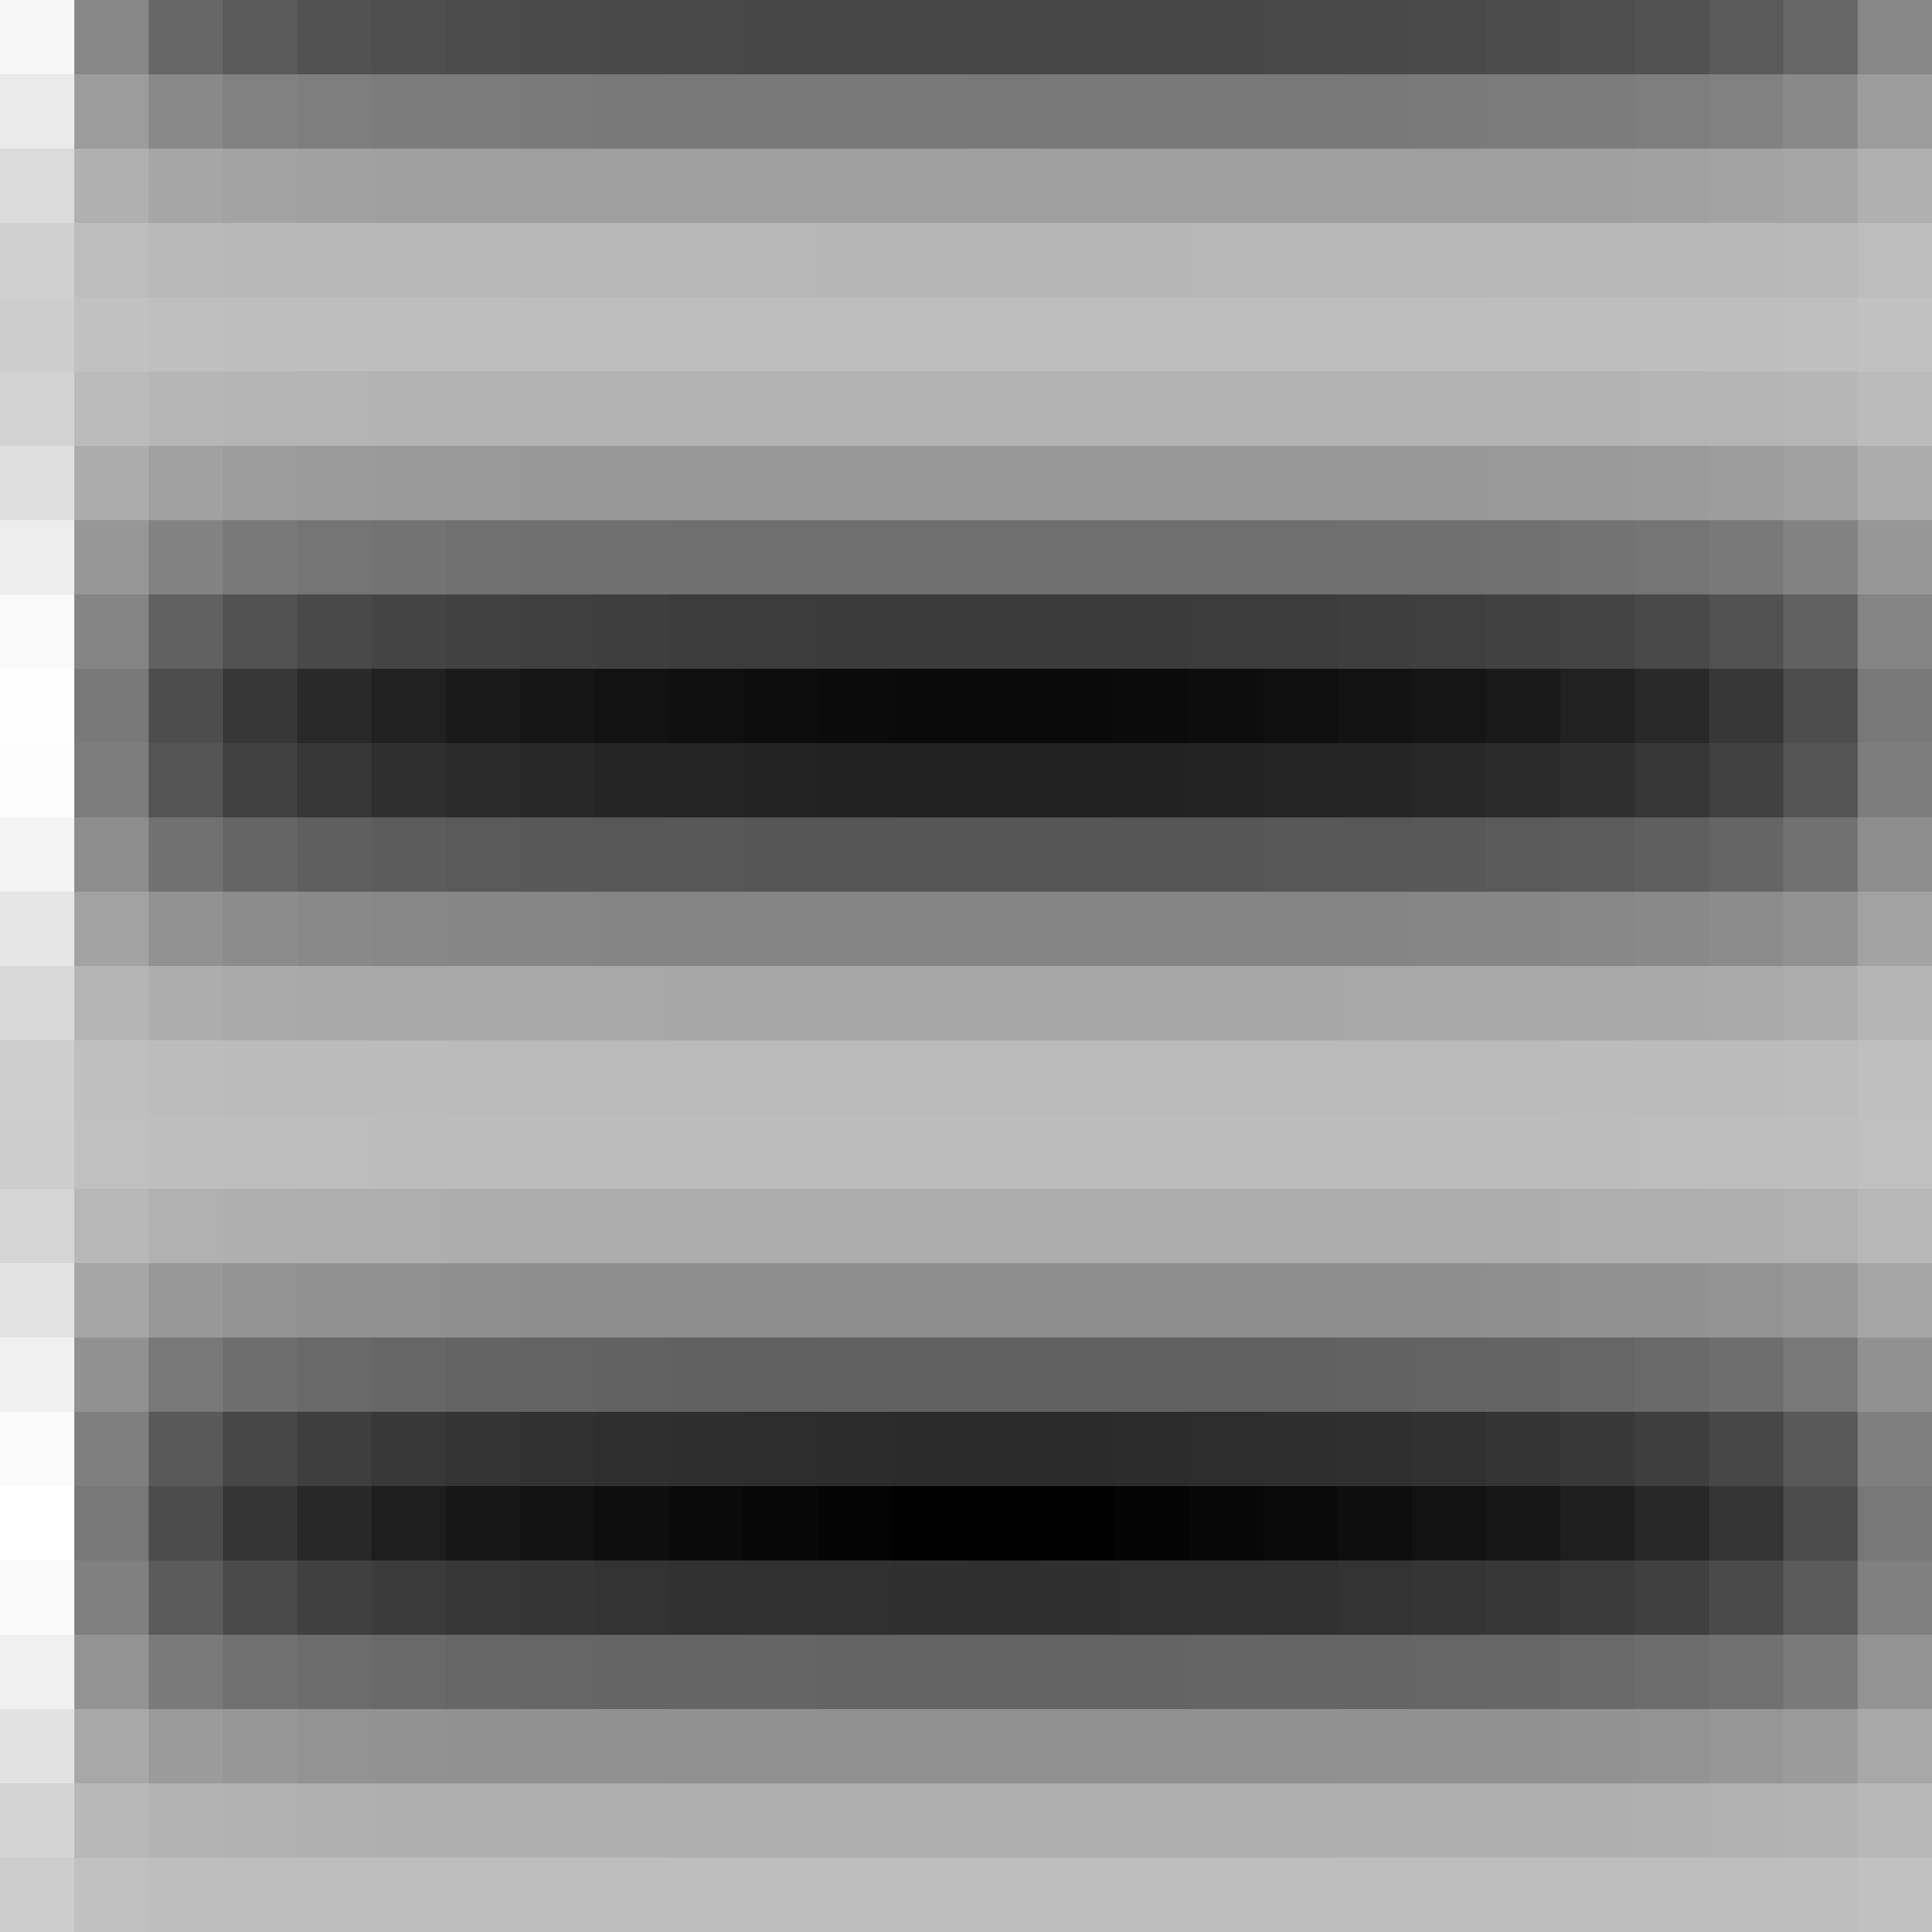
\includegraphics[width=40mm]{constante}
	            \caption{Representacion gráfica de una señal de frecuencia constante}
	            \label{imagen2}
	        \end{figure}
	
	        \begin{figure}[h!]
	            \centering
	            
\includegraphics[width=40mm]{variable}
	            \caption{Representación gráfica de una señal con variación de frecuencia lineal $y_{[n]} = sen(\frac{2\pi}{60}n^2)$}
	            \label{imagen3}
	        \end{figure}
	
	        \paragraph{}
	        Este procesamiento de los datos fue realizado con el fin de poder analizar más intuitivamente la información presentada, 
	        pudiendo así contrastar los diferentes escenarios conocidos contra la señal en estudio e identificar a cuál se asemeja.
	\subsection{Análisis de los resultados}
	        
	        %Luego de realizado el procesamiento de las imágenes, analizamos distintas funciones con distintas frecuencias y comportamientos para ayudarnos en el análisis de la señal en estudio. 
		Para ayudarnos en el análisis de la señal en estudio, procesamos de igual manera señales conocidas, para así comparar sus matrices de espectro con la de la señal en estudio. Pudimos conjeturar que los valores presentes en la matriz de espectro representan la concentración de 
	        energía en determinadas frecuencias de los valores que conforman los segmentos. Además, se pudo concluir que la señal propuesta 
	        se asemeja a una función que varía linealmente en frecuencia.
	        
	        Analizando más en detalle matrices de espectro con funciones de frecuencia linealmente variable, concluimos que a partir del muestreo de distintas funciones se observa un patrón, en el caso de funciones con frecuencias aptas para el muestreo (bajas frecuencias) se observan dos lineas de frecuencias predominantes. 
	        
	        
	          \begin{figure}[h!]
	            \centering
	            
\includegraphics[width=40mm]{variable15}
	            \caption{Representación gráfica de una señal con variación de frecuencia lineal $y_{[n]}= sen(\frac{2\pi}{15}n^2)$ }
	            \label{valor15}
	        \end{figure}
	        
	         \begin{figure}[h!]
	            \centering
	            
\includegraphics[width=40mm]{variable5}
	            \caption{Representación gráfica de una señal con variación de frecuencia lineal $y_{[n]} = sen(\frac{2\pi}{5}n^2)$ }
	            \label{valor5}
	        \end{figure}
	
	Se puede observar desde la figura \ref{imagen3} hasta la \ref{valor5}, que a medida que aumentamos la frecuencia, las lineas predominantes se interceptan. En las imágenes \ref{valor15} y \ref{valor5} se produce alliasing por el efectodel muestreo de seales de alta frecuencia. por lo tanto analizando la matriz de espectro de la señal en estudio podemos determinar que se produce alliasing y en consecuencia la discretización de la señal no fue buena.

\section{Sistema masa-resorte-amortiguador discreto}

Como contrapartida de la ecuación diferencial que modela el comportamiento del sistema en estudio, se desarrolla la ecuación en diferencias contemplando las siguientes aproximaciones:

$$y'_{(t)} \approx \frac{y_{[n+1]}-y_{[n-1]}}{2T}$$

$$y''_{(t)} \approx \frac{y_{[n+1]} - 2 y_{[n]} + y_{[n-1]}}{T^2}$$

siendo $T$ el tiempo entre muestras. Si bien no es posible interpretar la derivada de una función discreta en el tiempo, las expresiones mostradas son una aproximación.


Por lo tanto, para aproximar la ecuación diferencial que simula al sistema del amortiguador, debemos reemplazar todas las apariciones de $y'$ e $y''$.

Siendo el sistema contínuo del amortiguador:

$$k_3 y''_{(t)} + k_2 y'_{(t)} + k_1 y_{(t)} = x_{(t)}$$

Nos queda que la ecuación en diferencia que aproxima al modelado continuo del sistema sería:

$$k_1 y_{[n]} + k_2 \left(\frac{y_{[n+1]}-y_{[n-1]}}{2T}\right) + k_3 \left(\frac{y_{[n+]1} - 2 y_{[n]} + y_{[n-1]}}{T^2}\right)= x_{[n]}$$

A partir de esta ecuación en diferencias se puede calcular la función de tranferencia del sistema, quedando la misma:

$$H_{(z)} = \frac{1}{\left(\frac{k_3}{T^2} - \frac{k_2}{2T}\right) z^{-1} + \left(k_1-\frac{2k_3}{T^2}\right) + \left(\frac{k_2}{2T} + \frac{k_3}{T^2}\right) z} $$


Reemplazando los valores de $k_1$, $k_2$, y $k_3$ por los correspondientes a la entrega anterior, y definiendo $T=0.1$ obtendríamos una discretización del sistema estudiado, obteniendo valores con una frecuencia de 10 Hz. De esta manera podemos reconstruir cualuier señal con un ancho de banda menor a 5 Hz, debido a que el amortiguador es un sistema mecánico suponemos que  no existirán variaciones de mayor frecuencia que esta.

$$ k_1 =1$$
$$k_2 =10$$
$$k_3=1$$

De esta manera contrastar la respuesta del sistema contínuo y la discretización resultante en este ejercicio.

        \begin{figure}[h!]
            \centering
            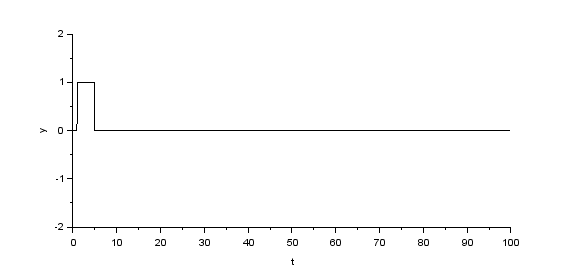
\includegraphics[width=0.7\textwidth]{amortiguador_entrada.png}
            \caption{Entrada del sistema.}
            \label{entrada}
        \end{figure}
        
         \begin{figure}[h!]
            \centering
            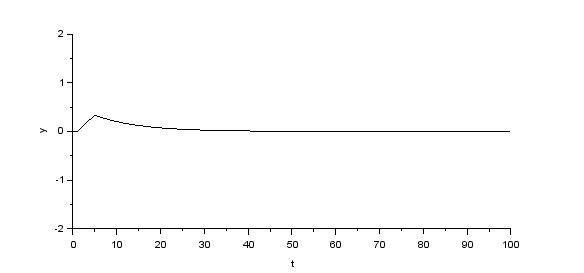
\includegraphics[width=0.7\textwidth]{amortiguador_10}
            \caption{Salida resultante de simular el sistema con un sistema LTI contínuo.}
            \label{sistemaContinuo}
        \end{figure}
        
              \begin{figure}[h!]
            \centering
            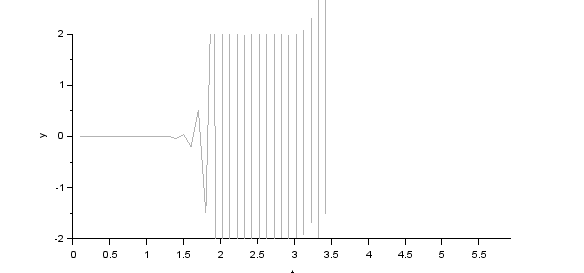
\includegraphics[width=0.7\textwidth]{discreto.png}
            \caption{Salida resultante de simular el sistema con un sistema LTI discreto.}
            \label{sistemaDiscreto}
        \end{figure}

Como se observan en las imágenes, la discretización elegida no resulta útil para el estudio del sistema, ya que no existe una clara relación con su contraparte contínua. Esto deja en evidencia que el muestreo elegido no fue adecuado. Posiblemente se logren mejores aproximaciones utilizando frecuencias de muestreo mayores.








    
\end{document}

